\subsection{ADD/SUB}

\begin{frame}
    \frametitle{ADD/SUB}
    A selector cand be done such that any of $ADD$ or $SUB$ can be performend with the same hardware in the case of two's complement.
    Let's consider the following notations for the operands $x$ and $y$.
    \begin{equation}
        \begin{aligned}
            &result=
                \begin{cases}
                    x+y,& \text{if ADD}\\
                    x+(-y), & \text{if SUB}
                \end{cases}
        \end{aligned}
    \end{equation}
\end{frame}

\begin{frame}
    \frametitle{ADD/SUB}
\end{frame}

\begin{frame}
    \frametitle{Adder}
    Type of adder implementations in hardware are:
    \begin{itemize}
        \item Ripple Carry Adder
        \item Carry Lookahead Adder
            \begin{itemize}
                \item Carry Skip Adder (bypass)
                \item Carry Select Adder (multiplexer)
            \end{itemize}
    \end{itemize}
\end{frame}

\begin{frame}
    \frametitle{Half adder}
    A half adder is a combinational circuit that adds two bits and produces a sum bit and a carry bit.
    \begin{figure}
        \centering
        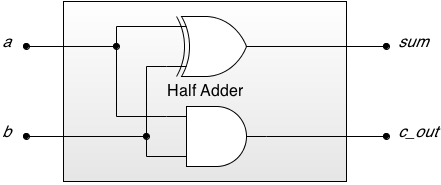
\includegraphics[width=0.7\textwidth]{media/half-adder-gates.png}
        \caption{Half Adder}
    \end{figure}
\end{frame}

\begin{frame}
    \frametitle{Full adder}
    A full adder is a combinational circuit that adds three bits and produces a sum bit and a carry bit.
    \begin{figure}
        \centering
        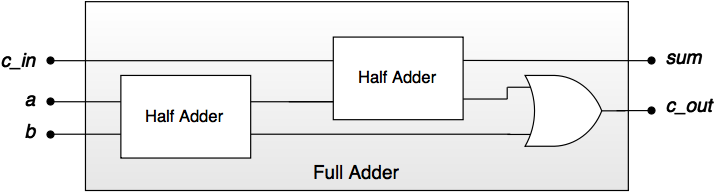
\includegraphics[width=0.7\textwidth]{media/full-adder-gates.png}
        \caption{Full Adder}
    \end{figure}
\end{frame}

\begin{frame}
    \frametitle{Ripple Carry Adder}
    The simplest adder is the ripple carry adder. It is composed of a chain of full adders. The carry out of one full adder is the carry in of the next full adder.
    \begin{figure}
        \centering
        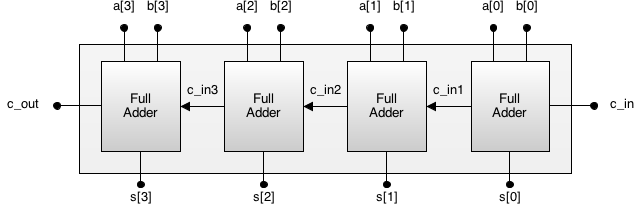
\includegraphics[width=0.7\textwidth]{media/ripple-carry.png}
        \caption{Ripple Carry Adder}
    \end{figure}
\end{frame}

\begin{frame}
    \frametitle{Let's do some math}
    \begin{equation}
        \begin{aligned}
            &sum[0]=a[0] \oplus b[0] \oplus c_{in}[0]\\
            &c_{in}[1]=c_{out}[0]=a[0]\ \& \ b[0] \ | \ c_{in}[0] \ \& \ (a[0] \oplus b[0])\\
            &sum[i]=a[i] \oplus b[i] \oplus c_{in}[i]\\
            &c_{in}[i+1]=c_{out}[i]=a[i] \ \& \ b[i] \ | \ c_{in}[i] \ \& \ (a[i] \oplus b[i])\\
            &G[i]=a[i] \ \& \ b[i]\\
            &P[i]=a[i] \oplus b[i]\\
            &c_{in}[i+1]=c_{out}[i]=G[i] \ | \ c_{in}[i] \ \& \ P[i]
        \end{aligned}
    \end{equation}
\end{frame}


\begin{frame}
    \frametitle{Let's do some math}
    \begin{equation}
        \begin{aligned}
            & \text{Ripple Carry Adder number of gates for carry out: } 3 \times n\\
            & \text{Carry Lookahead Adder number of gates for carry out: } 2 \times n\\
        \end{aligned}
    \end{equation}
\end{frame}


\begin{frame}
    \frametitle{Carry Lookahead Adder}
    The carry lookahead adder is a more complex adder that reduces the time to calculate the carry out of each full adder. It is composed of two main blocks:
    \begin{itemize}
        \item Generate block
        \item Propagate block
    \end{itemize}
    The carry out and sum of each full adder is calculated by the following formula:
    \begin{equation}
        \begin{aligned}
            &c_{out}[i]=G[i] \ | \ P[i] \ \& \ c_{in}[i]\\
            &sum[i]=P[i] \oplus c_{in}[i]
        \end{aligned}
    \end{equation}

\end{frame}

\begin{frame}
    \frametitle{Carry Lookahead Adder}
    \begin{figure}
        \centering
        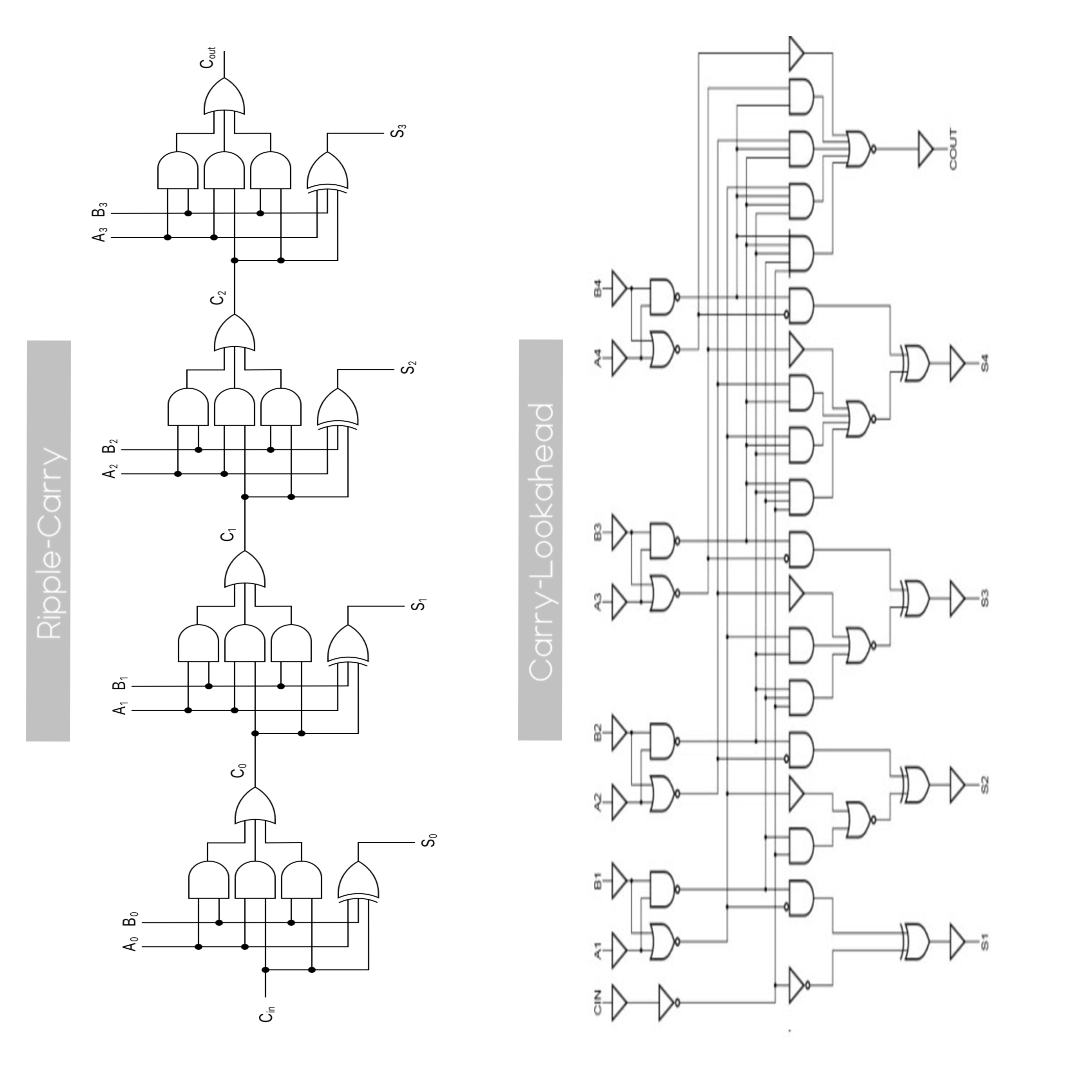
\includegraphics[width=0.5\textwidth, angle=270 ]{media/adders_comparison.jpg}
        \caption{Carry Lookahead Adder vs Ripple Carry Adder}
    \end{figure}
\end{frame}

\begin{frame}
    \frametitle{Let's do some math}
    \begin{equation}
        \resizebox{0.9\textwidth}{!}{%
            $
            \begin{aligned}
                &c_{in}[i+1]=c_{out}[i]=G[i] \ | \  P[i] \ \& \ c_{in}[i]\\
                &c_{in}[i+1]=G[i] \ | \  P[i] \ \& \ (G[i-1]  \ | \  P[i-1] \ \& \ c_{in}[i-1])\\
                &c_{in}[i+1]=G[i] \ | \  P[i] \ \& \ (G[i-1]  \ | \  (P[i-1] \ \& \ (G[i-2]  \ | \  P[i-2] \ \& \ c_{in}[i-2])))\\
                &c_{in}[i+1]=G[i] \ | \  (P[i] \ \& \ G[i-1])  \ | \  (P[i] \ \& \ P[i-1] \ \& \ (G[i-2]  \ | \  P[i-2] \ \& \ c_{in}[i-2]))\\
                &c_{in}[i+1]=G[i] \ | \  (\sum_{j=1}^{i} (\prod_{k=i}^{j} P[k]) \  \& \ G[j-1]) \ | \  ((\prod_{k=0}^{i} P[k]) \ \& \ c_{in}[0])\\
            \end{aligned}$%
        }
    \end{equation}
\end{frame}

\subsection{MUL}

\subsection{DIV/MOD}

\subsection{ROOT}

\subsection{POWER}
